\documentclass[11pt, oneside]{article}   	% use "amsart" instead of "article" for AMSLaTeX format
\usepackage{geometry}                		% See geometry.pdf to learn the layout options. There are lots.
\geometry{letterpaper}                   		% ... or a4paper or a5paper or ... 
%\geometry{landscape}                		% Activate for for rotated page geometry
%\usepackage[parfill]{parskip}    		% Activate to begin paragraphs with an empty line rather than an indent
\usepackage{graphicx}				% Use pdf, png, jpg, or eps� with pdflatex; use eps in DVI mode
								% TeX will automatically convert eps --> pdf in pdflatex		
\usepackage{amssymb}
\usepackage{amsmath}
\usepackage{parskip}
\usepackage{color}
\usepackage{hyperref}

\title{Integrating z}
%\author{The Author}
%\section{}
%\subsection*{}
\date{}							% Activate to display a given date or no date

\graphicspath{{/Users/telliott_admin/Dropbox/Tex/png/}}
% \begin{center} 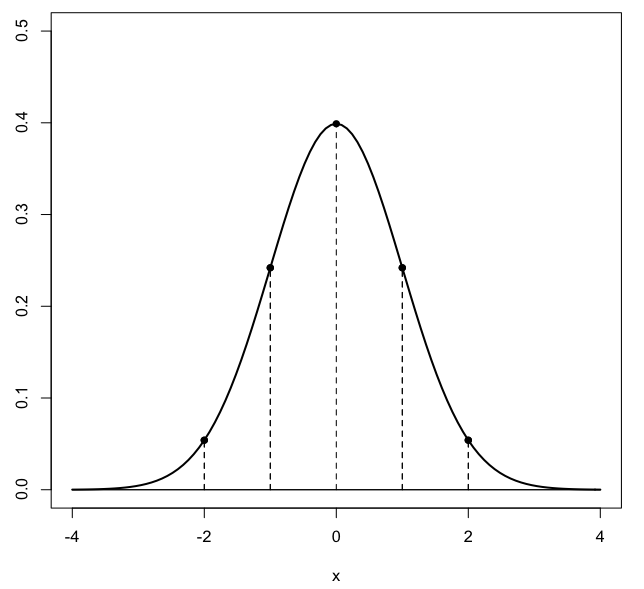
\includegraphics [scale=0.4] {gauss3.png} \end{center}
\begin{document}
\maketitle
\Large
Suppose $f(z) = z$, so we want
\[ f(z) = u(x,y) + i v(x,y) = x + iy \]
Write
\[ I = \int u \ dx - \int v \ dy + i \ [ \ \int v \ dx + \int u \ dy \ ] \]
\[ I = \int x \ dx - \int y \ dy + i \ [ \ \int y \ dx + \int x \ dy \ ] \]

Suppose the path proceeds from the origin to the point $(1,1)$ either directly ($C_1$) or first horizontally out to $(1,0)$ ($C_2$) and then vertically ($C_3$).

Along $C_1$ we parametrize as follows:  $y=x=t$, $t = 0 \rightarrow 1$,  so $dy = dx = dt$ and we have
\[ I = \int t \ dt - \int t \ dt + i \ [ \ \int t \ dt + \int t \ dt \ ] \]
\[ = 2 i \ \int_0^1 t \ dt = 2i \ \frac{t^2}{2} \ \bigg |_0^1 = i \]
Along $C_2$, $y=0$, $dy=0$, $x=0 \rightarrow 1$ so
\[ = \int x \ dx - \int y \ dy + i \ [ \ \int y \ dx + \int x \ dy \ ] \]
\[ = \int x \ dx = \frac{x^2}{2} \ \bigg |_0^1 = \frac{1}{2} \]
Along $C_3$, $x=1$, $dx=0$, $y=0 \rightarrow 1$ so
\[ = \int x \ dx - \int y \ dy + i \ [ \ \int y \ dx + \int x \ dy \ ] \]
\[ = - \int y \ dy + i \ \int 1 \ dy \]
\[ = - \frac{y^2}{2} + i y \  \bigg |_0^1 = - \frac{1}{2} + i \]
Notice that
\[ I_{C1} = I_{C2} + I_{C3} = i \]
and a closed path where we return to the origin would be zero.

Also, since $f(z)$ is analytic, we can just do
\[ \int_{0 + 0i}^{1 + i} z \ dz = \frac{z^2}{2}  \  \bigg |_{0 + 0i}^{1 + i} \]
\[ = \frac{1}{2} \ (1+i)^2 = \frac{1}{2} \ (1 + i)(1 + i) = \frac{1}{2} \ (1 - 1 + 2i) = i \]

Let's try another path:  the unit circle, going counter-clockwise.  Write:
\[ z = e^{i\theta}, \ \ \ dz = i e^{i \theta} d \theta \]
\[ \oint f(z) \ dz = i \ \int_0^{2\pi} e^{i2\theta} \ d \theta \]
\[ = i \ \frac{1}{2i} e^{i2\theta}  \  \bigg |_0^{2\pi} = \frac{1}{2} \ (1 + i0 - 1 - i0) = 0 \]

\end{document}  